\documentclass[]{article}
\usepackage{amsmath}\usepackage{amsfonts}
\usepackage[margin=1in,footskip=0.25in]{geometry}
\usepackage{mathtools}
\usepackage{hyperref}
\hypersetup{
	colorlinks=true,
	linkcolor=blue,
	filecolor=magenta,
	urlcolor=cyan,
}
\usepackage[final]{graphicx}
\usepackage{listings}
\usepackage{courier}
\lstset{basicstyle=\footnotesize\ttfamily,breaklines=true}

% \usepackage{wrapfig}
\graphicspath{{.}}

\begin{document}
\begin{center}
	CSE 546 SPRING 2021: HW1 
\end{center}
\begin{center}
	Name: Honda Li
\end{center}

\section*{Bias-Variance tradeoff}
	\subsubsection*{B.1.a}
		\hspace{1.1em}
		When $m$ is relative small (Relative to the observed samples), the variance will be huge, and when the value of $m$ is huge, then the bias will be huge. 
		\par
		When $m = 1$, the function $\hat{f}(x)$ got decay into a k-nn method that checks of the closest labor. The model is literally looking for the $\hat{y}$ by looking for $x_i$ that is closest to the test sample. This will produce a great amount of variance, and the more sample there is, the more variance we have for the estimated model. 
		\par
		When $m = n$, we have $\hat{f}(x)$ returning the average of the samples, regardless of what the input is. This means that as we have more and more sample, the average will converge. Meaning all estimated models converge to one model. But the bias is not reduced because some ground truths might not be a horizontal line. 
	\subsubsection*{B.1.b}
		\hspace{1.1em}
		We defined $\bar{f}^{(j)}=\frac{1}{m}\sum_{i = (j - 1)m + 1}^{jm}f\left(x_i\right)$, which is just the average of the ground truth function $f(x)$ over the $j$ th partition. 
		\par
		\textbf{Objective: } figure out the Bias-squared as: $\frac{1}{n}\sum_{i = 1}^{n}\left(\mathbb{E}\left[\hat{f}_m(x_i)\right] - f(x_i)\right)^2$. 
		\par
		Let's start by considering the quantity: $\mathbb{E}\left[\hat{f}_m(x_i)\right]$. 
		\begin{align*}\tag{B.1.b.1}\label{eqn:B.1.b.1}
			\mathbb{E}\left[\hat{f}_m(x_i)\right] \underset{(1)}{=}&
			\mathbb{E}\left[c_{\left\lceil\frac{i}{m}\right\rceil}\right]
			\\
			\mathbb{E}\left[c_{\left\lceil\frac{i}{m}\right\rceil}\right]
			=& 
			\frac{1}{m}\sum_{i=(j - 1)m + 1}^{jm}\mathbb{E}\left[\underbrace{f(x_i) + \epsilon}_{y_i}\right]
			\text{where } \quad  j = 
			\left\lceil\frac{i}{m}\right\rceil
			\\
			=& 
			\frac{1}{m}\sum_{i=(j - 1)m + 1}^{jm}f(x_i) 
			\\
			=&
			\bar{f}^{\left(
				\left\lceil\frac{i}{m}\right\rceil
			\right) }
		\end{align*}
		(1): Because, for any $x_i$, it will only fall onto one of the partition, and the partition is $\left\lceil \frac{i}{m}\right\rceil$. This true because $x_i = \frac{i}{n}$ and $i\in\mathbb{N}$. So the index of the sample tells us which interval it's falling onto and what the value of $j$ is going to be for that sample $x_i$. Hence, it set all other $c_j$ to zeroes, except when $j = \left\lceil\frac{i}{m}\right\rceil$
		\\[1em]
		Now, we consider the Bias-squared in this way: 
		\begin{align*}\tag{B.1.b.2}\label{eqn:B.1.b.2}
			\frac{1}{n}\sum_{i = 1}^{n}\left(\mathbb{E}\left[\hat{f}_m(x_i)\right] - f(x_i)\right)^2
			=&
			\frac{1}{n}\sum_{i = 1}^{n}\left(
				\bar{f}^{\left\lceil\frac{i}{m}\right\rceil}
				-
				f(x_i)
			\right)^2
			\\
			\underset{(2)}{=}&
			\frac{1}{n}\sum_{j = 1}^{n/m}\sum_{i = (j - 1)m - 1}^{jm}\left(
				\bar{f}^{(j)} - f(x_i)
			\right)^2
		\end{align*}
		(2): This is true because, there is a group of indices $i$ that is going to fall under the $j$ th groups, and those indices are in the range of $i \in \mathbb{N}\cap [(j - 1)m - 1, jm]$ and for all such index $i$, the value of $\bar{f}^{\left\lceil\frac{i}{m}\right\rceil}$ is going to be the same. Because we rounded the fraction $\frac{i}{m}$.
	\subsubsection*{B.1.c}
		\hspace{1.1em}
		Let's dive into the math starting with the given definition of average variance in the problem statement, which is: 
		\par
		\begin{align*}\tag{B.1.c.1}\label{eqn:B.1.c.1}
			& \mathbb{E}\left[
				\frac{1}{n}
				\sum_{i = 1}^{n}\left(
					\hat{f}_m(x_i) - \mathbb{E}\left[\hat{f}_m(x_i)\right]
				\right)^2
			\right] 
			\\=& 
			\frac{1}{n}
			\sum_{i = 1}^{n}
			\mathbb{E}\left[
				\left(
					\hat{f}_m(x_i) - \mathbb{E}\left[\hat{f}_m(x_i)\right]
				\right)^2
			\right]
			\\
			=&
			\frac{1}{n}\sum_{j = 1}^{n/m}\sum_{i = (j - 1)m + 1}^{mj}
			\mathbb{E}\left[
				\left(
					\hat{f}_m(x_i) - \mathbb{E}\left[\hat{f}_m(x_i)\right]
				\right)^2
			\right]
		\end{align*}
		Let's pause for a moment and think about the fact that, the outter sum is summing over each of the partition. And we know that for all $i\in \mathbb{N}\cap[(j - 1)m + 1, jm]$, which is just all the indices for the sample that are presented in the $j$ th partition, the value of $\hat{f}_m(x_i)$ and the value of $\mathbb{E}\left[\hat{f}_m(x_i)\right]$ is going to be the same and they are: $c_j$ and $\bar{f}^{(j)}$. 
		\begin{align*}\tag{B.1.c.2}\label{eqn:B.1.c.2}
			\frac{1}{n}\sum_{j = 1}^{n/m}\sum_{i = (j - 1)m + 1}^{mj}
			\mathbb{E}\left[
				\left(
					\hat{f}_m(x_i) - \mathbb{E}\left[\hat{f}_m(x_i)\right]
				\right)^2
			\right] 
			= &
			\frac{1}{n}\sum_{j = 1}^{n/m}\sum_{i = (j - 1)m + 1}^{mj}
			\mathbb{E}\left[
				\left(
					c_j - \bar{f}^{(j)}
				\right)^2
			\right] 
			\\
			=& 
			\frac{1}{n}\sum_{j = 1}^{n/m}
				m\mathbb{E}\left[
					(c_j - \bar{f}^{(j)})^2
				\right] 
		\end{align*}
		And hence, we have proven the first equality stated in the problem. Next, let's observe the fact that $c_j$ is the average of all the samples over the $j$ th partition which is given as $\frac{1}{m}\sum_{i = (j - 1)m + 1}^{jm}y_i$ and in this case $y_i = f(x_i) + \epsilon$, but at the same time $\bar{f}^{(j)} = \frac{1}{m}\sum_{i = (j - 1)m + 1}^{mj}f(x_i)$ and hence we know that: $c_j - \bar{f}^{(j)} = \frac{1}{m}\sum_{i = (j - 1)m + 1}^{jm}\epsilon_i$, which is conveniently giving us the result that: 
		\begin{align*}\tag{B.1.c.3}\label{eqn:B.1.c.3}
			\frac{1}{n}\sum_{j = 1}^{n/m}
			m\mathbb{E}\left[
				(c_j - \bar{f}^{(j)})^2
			\right]
			&=
			\frac{1}{n}\frac{n}{m}m \mathbb{E}\left[
				\left(
					\frac{1}{m}\sum_{i = (j - 1)m + 1}^{jm}\epsilon_i
				\right)^2
			\right]
			\\
			&= \mathbb{E}\left[
				\left(
					\frac{1}{m}\sum_{i = 1}^{m}\epsilon_i
				\right)^2
			\right]
		\end{align*}
		Let's pause for a moment and remember that $\epsilon \sim \mathcal{N}(0, \sigma^2)$, and in this case, we take the average for $m$ of them, hence, $\frac{1}{m}\sum_{i = `'}^{m}\epsilon_i\sim \mathcal{N}(0, \sigma^2/m)$. 
		\\
		However, we also need to note that for any Gaussian Random variable say: $X\sim \mathcal{N}(0, \sigma^2)$, the variance $\sigma^2 = \mathbb{E}\left[X^2\right] - \mathbb{E}\left[X\right]^2$(The mean is zero!) which implies that $\mathbb{E}\left[X^2\right] = \sigma^2$. Hence, combining this fact and the previous statement (Basically $X = \frac{1}{m}\sum_{i = 1}^{m}\epsilon_i$), we know that: 
		\begin{equation*}\tag{B.1.c.4}\label{eqn:B.1.c.4}
			\mathbb{E}\left[
				\left(
					\frac{1}{m}\sum_{i = 1}^{m}\epsilon_i
				\right)^2
			\right] = \frac{\sigma^2}{m}
		\end{equation*}
	\subsubsection*{B.1.d}
		Programming Part. Here is the Plot I got: 
		\begin{center}
			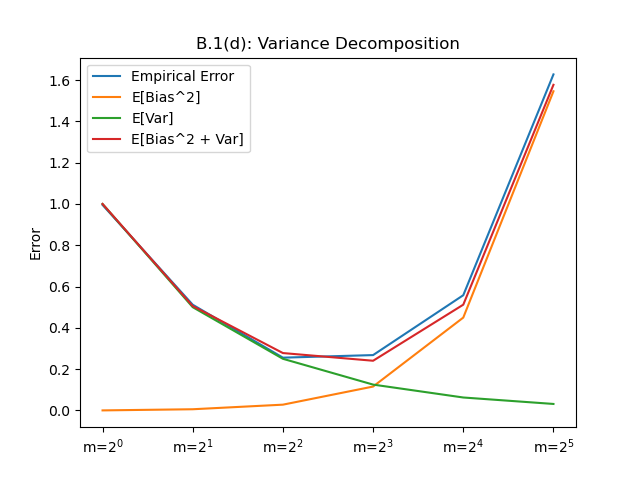
\includegraphics[width=8cm]{B.1(d)plot.png}
		\end{center}
		And this is the code I used to generate the graph: 
		\begin{lstlisting}[language=python]
# Code is for B1(d), HW1, CSE 546.
import numpy as np
sin    = np.sin
cos    = np.cos
array  = np.array
PI     = np.pi
rnd    = np.random.normal
arange = np.arange

import math
ceil  = math.ceil
zeros = np.zeros
mean  = np.mean

import matplotlib.pyplot as plt
scatter = plt.scatter
plot    = plt.plot
show    = plt.show
xticks  = plt.xticks
title   = plt.title
legend  = plt.legend
save    = plt.savefig
ylabel  = plt.ylabel

def f(x):
	return 4*sin(x*PI)*cos(6*PI*x)


def Epsilon(length):
	return rnd(0, 1, length)


def GenerateData(n=256):
	Xgrid = array([(II + 1)/n for II in range(n)])
	return Xgrid, f(Xgrid) + Epsilon(n)


def yHat(data, m, n=256):
	"""
		Given the data, fit it with average data points on each of the partition.
	Args:
		data:
		m:
		n:
	Returns:
		Predicted value
	"""
	y = zeros(n)
	for JJ in range(int(n/m)):
		UpperBound = min((JJ + 1)*m, n)
		LowerBound = JJ*m
		y[LowerBound: UpperBound] = mean(data[LowerBound: UpperBound])
	return y


def fBar(xgrid, m, n=256):
	return yHat(f(xgrid), m, n)


def AvgBiasSqaured(m, n=256):
	"""
		The expected vaue of the biases error squared. Because it's expected value,
		this will use the underlying generative model instead of using data to get
		the error from the biases squared.

	Args:
		data:

	Returns:

	"""
	Xgrid = array([(II + 1)/n for II in range(n)])
	FBar  = fBar(Xgrid, m, n)
	F     = f(Xgrid)
	return mean((FBar - F)**2)


def AvgVariance(m):
	return 1/m


def AvgEmpiricalErr(yhat, n=256):
	Xgrid = array([(II + 1)/n for II in range(n)])
	return mean((f(Xgrid) - yhat)**2)


def main():
	def FitDemo():
		Xs, Ys = GenerateData()
		scatter(Xs, Ys)
		Yhat = yHat(Ys, 8)
		YBar = fBar(Xs, 8)
		plot(Xs, Yhat, c="red")
		plot(Xs, YBar, c="green")
		show()
	FitDemo()
	def PlotErrors():
		Error1 = [] # Empirical error from 256 random samples.
		Error2 = [] # Expected Bias Squared
		Error3 = [] # Expcted Variance Square
		Error4 = [] # Expected Errors
		_, SampledData = GenerateData()
		for m in [2**II for II in range(6)]:
			Error1.append(AvgEmpiricalErr(yHat(SampledData, m)))
			Error2.append(AvgBiasSqaured(m))
			Error3.append(AvgVariance(m))
			Error4.append(Error2[-1] + Error3[-1])
		plot(Error1)
		plot(Error2)
		plot(Error3)
		plot(Error4)
		xticks(range(6), [f"m=$2^{II}$" for II in range(6)])
		ylabel("Error")
		legend(["Empirical Error", "E[Bias^2]", "E[Var]", "E[Bias^2 + Var]"])
		title("B.1(d): Variance Decomposition")
		save("B.1(d)plot.png")

	PlotErrors()


if __name__ == "__main__":
	import os
	print(f"wd: {os.getcwd()}")
	print(f"script running on{os.curdir}")
	main()
		\end{lstlisting}
	\subsubsection*{B.1.e}
		The mean value theorem asserts that: 
		\begin{align*}\tag{B.1.e.1}\label{eqn:B.1.e.1}
			\min_{(j - 1)m + 1\le i\le jm} f(x_i)\le 
			\bar{f}^{(j)}
			\le \max_{(j - 1)m +1\le i \le jm} f(x_i)
			\quad \forall 1 \le j \le \frac{n}{m}
		\end{align*}
		And the definition of the L-Lipschitz Continuity, we know that: 
		\begin{align*}\tag{B.1.e.2}\label{eqn:B.1.e.2}
			|f(x_i) - f(x_j)| \le& \frac{L}{n}|i - j| ;\quad \forall 1 \le i,j \le n
			\\
			\implies
			\left(
				\max_{(j - 1)m + 1\le i \le jm}
				\left(
					f(x_i) 
				\right)
			\right)
			- 
			\left(
				\min_{(j - 1)m + 1\le i \le jm}
				(f(x_i))
			\right)
			\le& \frac{L}{n}(jm) - ((j-1)m + 1) = \frac{Lm}{n}
			;\quad \forall 1 \le j \le \frac{m}{n}
			\\
			\underset{\text{
				\hyperref[eqn:B.1.e.1]{B.1.e.1}
			}}{\implies}
			\max_{(j-1)m + 1 \le i \le jm}
			\left(
				\bar{f}^{(j)} - f(x_i)
			\right)
			\le&
			\frac{Lm}{n} ;\quad\forall 1 \le j \le \frac{m}{n}
			\\
			\implies
			\frac{1}{n}\sum_{j = 1}^{n/m}\sum_{i = (j - 1)m - 1}^{jm}\left(
				\bar{f}^{(j)} - f(x_i)
			\right)^2
			\le&
			\sum_{j = 1}^{\frac{n}{m}}
			\max_{(j-1)m + 1 \le i \le jm}
			\left(
				\bar{f}^{(j)} - f(x_i)
			\right)^2
			\in
			\mathcal{O}
			\left(
				\left(
					\frac{Lm}{n}
				\right)^2
			\right)
			\\
			\underset{
				\text{\hyperref[eqn:B.1.b.2]{B.1.b.2}}
				}
				{\implies}
			\frac{1}{n}\sum_{i = 1}^{n}\left(\mathbb{E}\left[\hat{f}_m(x_i)\right] - f(x_i)\right)^2
			\in&
			\mathcal{O}
			\left(
				\left(
					\frac{Lm}{n}
				\right)^2
			\right)
		\end{align*}
		And hence, we have an upper bound for the error of the Bias squared. Now, combining both type of error, the average Variance and the Bias squared, we have error in the form of: $\mathcal{O}(\frac{L^2m^2}{n^2} + \frac{\sigma^2}{m})$. 
		\\[1em]
		Let's take the derivative of the expression, set it to zero and solve for the optimal $m$ such that the sum of these 2 types of errors are minimized: 
		\begin{align*}\tag{B.1.e.3}\label{eqn:B.1.e.3}
			\partial_m 
			\left[ 
				\frac{L^2m^2}{n^2} + \frac{\sigma^2}{m}
			\right] &= 0
			\\
			\frac{2mL^2}{n^2} - \frac{\sigma^2}{m} &= 0
			\\
			\frac{2m^2L^2}{n^2} - \sigma^2 &= 0
			\\
			m &= \sqrt{\frac{\sigma^2 n^2}{L^2}}
			\\
			m &= \frac{\sigma n}{L}
		\end{align*}
		The optimal value for $m$ is $\frac{\sigma n}{L}$, where $L$ tells us how wiggly the distribution underlying generative function $f$ is, and $\sigma$ tells us how smeared out the function $f(x)$ due to Gaussian Noise. If the Gaussian Noise is huge compare to the the amount of wiggle the function has, then we should use large $m$ to minimize the error, otherwise, we should choose relatively small value for $m$. However, $m$ is proportional to $n$, the number of samples, this a result of $x_i = i/n$, if the samples are not event scatter on the grid point, this term will look different. 
\section*{Ridge Regression on MNIST}
	\subsection*{B.2}
		\subsection*{(a)}
			For this problem, 10 000 samples are selected from the training set for cross validation, the choice is made to reduce the running time of the program. This means that 8000 samples were used to train a model for 5 times and then 2000 were used to validate the models and get the error. Then the average of those errors are taken to compute the estimated error, the percentage of the labels that the model got wrong. 
			\\
			And then, it's trained on $p$ value that goes from $300$ to $3000$ at an increment of $100$, and it's been identified that the best $p$ parameter is $2900$, with an error rate of $14589999999999997$. 
			\\
			Here is a plot of my results: 
			\begin{center}
\includegraphics[width=10cm]{B2plot.png}\end{center}
			And we can see that the training error is decreasing relatively fast compare to the cross validation error. 
			\\
			And here is the code for generating the graph: 
			\begin{lstlisting}[language=python]
### This file constains code for solving HW1 B2 for class CSE 546/446 SPRING 2021.
from mnist import MNIST
import numpy as np
from scipy.linalg import pinvh
import matplotlib.pyplot as plt
arr = np.array
eye = np.eye
pinv = np.linalg.pinv
argmax = np.argmax
randn = np.random.normal
rand = np.random.rand
sqrt = np.sqrt
pi = np.pi
cos = np.cos
arange = np.arange
mean = np.mean
argmin = np.argmin

plot = plt.plot
show = plt.show
saveas = plt.savefig
legend = plt.legend
title = plt.title
ylabel = plt.ylabel
xlabel = plt.xlabel


def load_dataset():
	mndata = MNIST("./data/")
	X_train, labels_train = map(np.array, mndata.load_training())
	X_test, labels_test = map(np.array, mndata.load_testing())
	X_train = X_train/255
	X_test = X_test/255
	return X_train, X_test, labels_train, labels_test


def train(X, Y, reg_lambda):
	"""
	d: The number of features for each of the samples.

	Args:
		X: Should be a "n by d" matrix, with all the samples pack vertically as rows into the matrix.
		Y: Should be a "n by 10" matrix, comtaninig all the labels for the digits pack vertically as
		rows for the matrix.
		reg_lambda:
			This is the regularization constant for the system.
	Returns:
		The trained linear model for the system, should be a 784 by 10 matrix such that its
		transpose multiply by the
		feature vector will produce the label vector.

	"""
	Y = Y.astype(np.float64)
	return pinvh(X.T@X + reg_lambda*eye(X.shape[1]))@X.T@Y


def predict(W, Xnew):
	"""

	Args:
		W: Should be a d by 10 matrix, which is the linear model.
		Xnew: Should be a n by 784 matrix that contains all the samples we want to
		to predict with using this given model.
	Returns:
		A single vector containing all the digits predicted using this model.
	"""
	return argmax(W.T@Xnew.T, axis=0)


def KFoldGenerate(k, X, Y):
	"""
		Generate k folds of data for K fold validations. same as sk.learn.model_selection.

	Args:
		k: The numer of folds.
		X: The row data matrix with training data.
		Y: The label of the training data set.
	Yields:
		Each of the train and test set separate by this program.
	"""
	assert X.ndim == 2 and Y.ndim == 1 and X.shape[0] == Y.size,\
		"The row data matrix has to be 2d with a lable vecor that has compatible size"
	# Shuffle the data.

	N = X.shape[0]
	n = N/k  # Partition size, could be a float.
	for II in range(k):
		ValidatePartitionStart = int(II*n)
		ValidatePartitionEnd = int((II + 1)*n)
		Xvalidate = X[ValidatePartitionStart: ValidatePartitionEnd, :]
		Yvalidate = Y[ValidatePartitionStart: ValidatePartitionEnd]
		TrainIndices = [Row for Row in range(N) if (Row < ValidatePartitionStart or Row >= ValidatePartitionEnd)]
		Xtrain = X[TrainIndices, :]
		Ytrain = Y[TrainIndices]
		yield Xtrain, Xvalidate, Ytrain, Yvalidate


class FeaturesRemap:

	def __init__(this, p):
		this.G = randn(0, sqrt(0.1), (p, 784))
		this.b = rand(p, 1)*2*pi

	def __call__(this, X):
		"""
		This is the functional call implementation. It trans form the row data matrix to the new
		cosine feature space.
		Returns:
			The transformed feature using a given data set.
		"""
		return (cos(this.G@X.T + this.b)).T

def TestKfoldGenearate():
	X = randn(0, 1, (17, 3))
	Y = rand(17)
	for X1, X2, Y1, Y2 in KFoldGenerate(5, X, Y): print(X1, X2, Y1, Y2)


def main():
	X1, X2, Y1, Y2 = load_dataset()
	# Reduce size of the training set for speed, or else it takes too long to run.
	# training size is 10 000, so then cross set is going to be
	X1 = X1[::6, :]
	Y1 = Y1[::6]
	print(X1.shape) # (60000, 784)
	print(X2.shape) # (10000, 784)
	print(Y1.shape) # (60000, )
	print(Y2.shape) # (10000, )
	print(X1.dtype)
	print(X2.dtype)
	print(Y1.dtype)
	print(Y2.dtype)
	print("Ok we are ready to train the model and make prediction now. ")
	TestKfoldGenearate()
	print("Test finished... Time to train")

	## USE THIS!
	def TrainTheModel(X1, Y1):
		# transform the Y labels from vector into Y matrix.
		Y = (np.array([[II] for II in range(10)]) == Y1).astype(np.float)
		return train(X1, Y.T, reg_lambda=1e-4)

	def ErrorRate(y1, y2):
		return sum(y1 != y2)/y1.size

	Pdegreees = arange(300, 3000, 100)
	KfoldTrainErrorRate = []
	KfoldValidateErrorRate = []
	for p in Pdegreees:
		TrainErrorsRate, ValErrorsRate= [], []
		Mapper = FeaturesRemap(p)
		print(f"pvalue is: {p}")
		for Xtrain, Xvalidate, Ytrain, Yvalidate in KFoldGenerate(5, X1, Y1):
			Xtrain = Mapper(Xtrain); print(f"Xtrain Map: {Xtrain.shape}")
			Xvalidate = Mapper(Xvalidate); print(f"Xval Map: {Xvalidate.shape}")
			Model = TrainTheModel(Xtrain, Ytrain); print("Model Train")
			PredictTrain = predict(Model, Xtrain); print("Predict Train Labels")
			Predictval = predict(Model, Xvalidate); print("Predict val labels")
			TrainErrorsRate.append(ErrorRate(PredictTrain, Ytrain))
			ValErrorsRate.append(ErrorRate(Predictval, Yvalidate))
			print("one of the k-fold ends.")
		print(f"List of train error score: {TrainErrorsRate}")
		print(f"List of Val Error score: {ValErrorsRate}")
		KfoldTrainErrorRate.append(mean(TrainErrorsRate))
		KfoldValidateErrorRate.append(mean(ValErrorsRate))
	plot(Pdegreees, KfoldValidateErrorRate)
	plot(Pdegreees, KfoldTrainErrorRate)
	title("B2 Error rate")
	legend(["Kfold Validation Error rate", "kfold training error rate"])
	ylabel("Percentage of wrong label"); xlabel("P; row count of G matrix")
	MinPindex = argmin(KfoldValidateErrorRate)
	MinP = Pdegreees[MinPindex]
	MinValError = KfoldValidateErrorRate[MinPindex]
	print(f"The best P is: {MinP}")
	print(f"The corresponding validation error is: {MinValError}")
	plot(MinP, MinValError, "bo")
	saveas("B2plot.png", format="png")




if __name__ == "__main__":
	import os
	print(f"cwd: {os.getcwd()}")
	print(f"script running at {os.curdir}")
	main()

			\end{lstlisting}
		\subsection*{(b)}
			The Hoeffding's Inequality is given as the following: 
			\begin{align*}\tag{B.2.1}\label{eqn:B.2.1}
			\end{align*}
			Assume that $X_i$ is the ith random variable draw from a Bernoulli Distribution, representing whether the model has gotten the $i$ th label correctly predicted in the validation set.  

		 

\end{document}
